\chapter{Lattice Vibrations and Phonons}

\section{Introduction}
In a crystalline material, atoms are not fixed at rigid lattice sites but vibrate around their equilibrium positions. One of the most important scattering mechanisms for mobile carriers in semiconductors arises from these lattice vibrations. \\
In the earlier discussion on bandstructure, we assumed that the background potential is perfectly periodic and time-independent. However, in real materials, the ions that constitute the crystal lattice are dynamic and undergo thermal vibrations, which become more pronounced with increasing temperature.\\
Scattering results from the disturbances in the periodic potential caused by lattice vibrations. \\
Before addressing how these vibrations lead to scattering, it is essential to first understand the fundamental properties of lattice vibrations themselves. Once these properties are established, we can then analyze how the resulting potential fluctuations contribute to carrier scattering in semiconductors.
\begin{center}
	\begin{minipage}{0.6\textwidth}
		\centering
		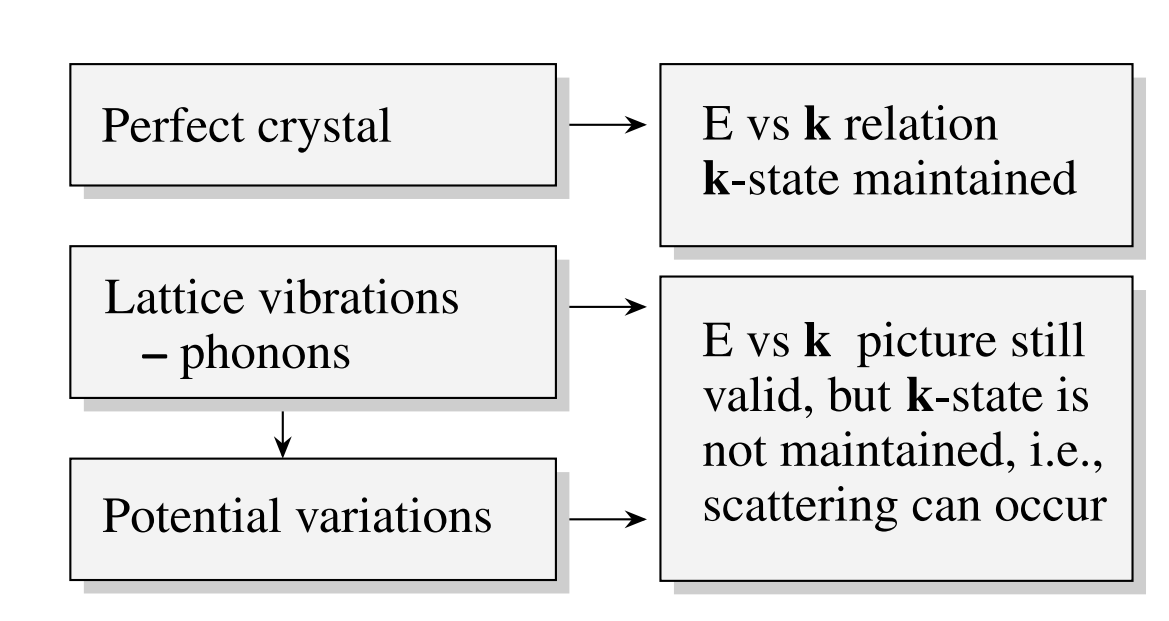
\includegraphics[width=\textwidth]{img/lattice_vibration_effects.png}
		\\[0.5em]
		\refstepcounter{figure}
		\textbf{Figure~\thefigure.}Electron scattering arises from imperfections in the crystal, including lattice vibrations (phonons) and local potential variations, which disrupt coherent transport.
		\label{fig:Lattice_vibration_effects}
	\end{minipage}
\end{center}


\section{Lattice Vibrations}
The reason a particular crystal structure is chosen by a material is fundamentally related to the minimization of the system’s total energy. As atoms approach each other to form a crystal, they experience both attractive and repulsive interactions. The attractive forces can arise from various mechanisms, such as Van der Waals interactions (due to induced dipole moments when electron clouds are perturbed by nearby atoms), ionic bonding (involving electron transfer between atoms), and covalent bonding (where electrons are shared between atoms).\\
When atoms are brought very close, however, there is a strong repulsive interaction primarily due to the Pauli exclusion principle, which prevents electrons on neighboring atoms from occupying the same space.\\
As a result, the total potential energy of the system as a function of interatomic separation exhibits a minimum at some equilibrium spacing \( R_0 \), where the system achieves mechanical stability.

In general, we can expand the crystal binding energy around the equilibrium spacing \( R_0 \) as a Taylor series:
\begin{equation}
	U(R) = U(R_0) + \left.\frac{dU}{dR}\right|_{R_0} \Delta R + \frac{1}{2} \left.\frac{d^2 U}{dR^2}\right|_{R_0} (\Delta R)^2 + \cdots
\end{equation}
\noindent
where \( \Delta R = R - R_0 \) is the deviation from equilibrium.
\begin{center}
	\begin{minipage}{0.6\textwidth}
		\centering
		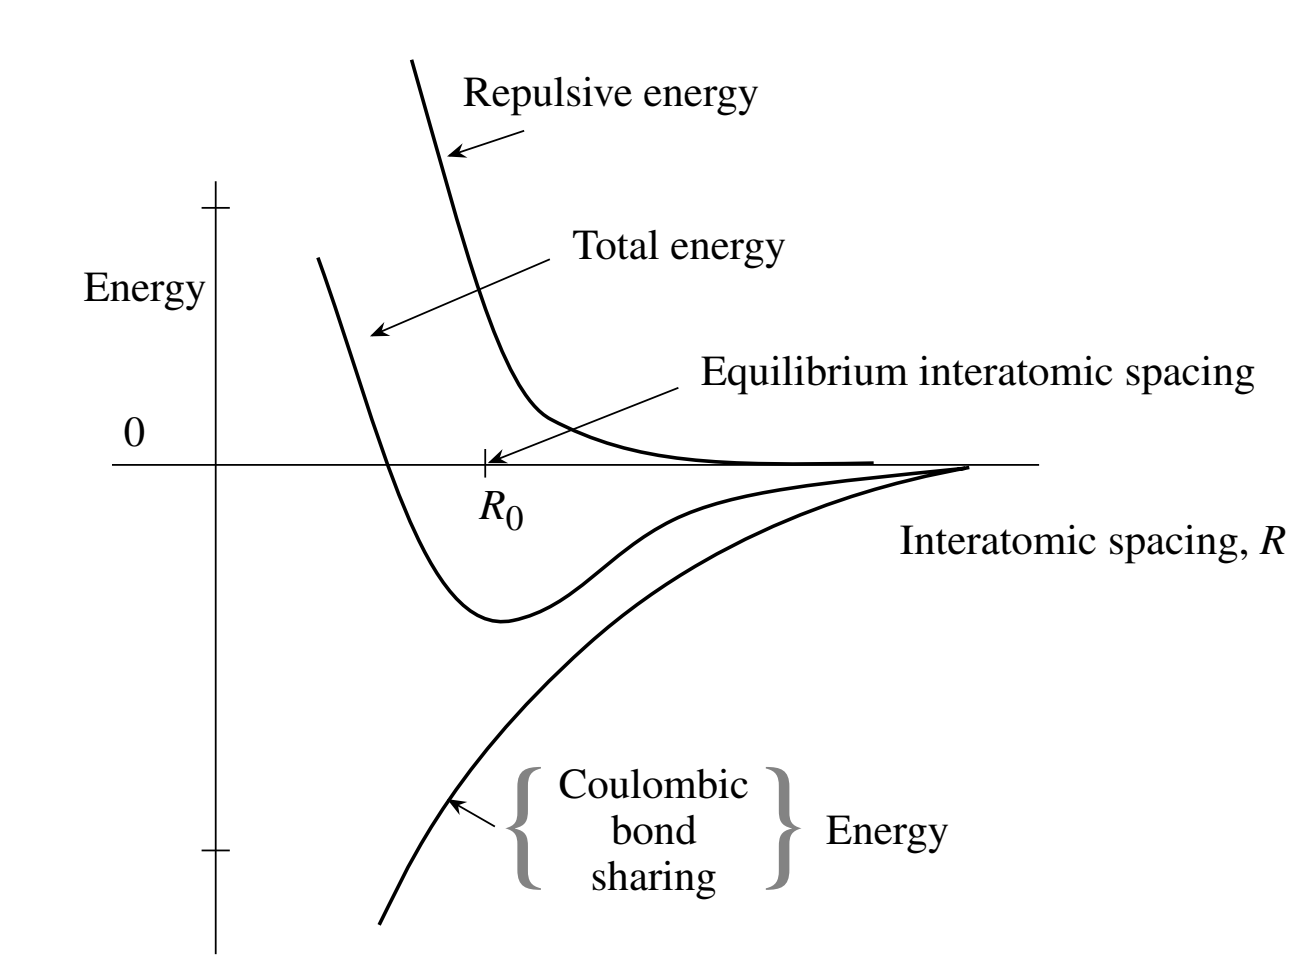
\includegraphics[width=\textwidth]{img/Potential_Energy.png}
		\\[0.5em]
		\refstepcounter{figure}
		\textbf{Figure~\thefigure.}General relationship between binding energy and atomic separation in a crystal. In semiconductors, long-range attraction typically arises from electrostatic interactions or covalent bond energy associated with electron sharing.
		\label{fig:Potential_Energy}
	\end{minipage}
\end{center}
The second term in the expansion is zero since \( R_0 \) is the equilibrium interatomic separation. Retaining terms up to second order in \( \Delta R \), we obtain what is known as the \textit{harmonic approximation}:
\begin{equation}
	U(R) = U(R_0) + \frac{1}{2} C (\Delta R)^2
\end{equation}
where the force constant \( C \) is given by:
\begin{equation}
	C = \left. \frac{\partial^2 U}{\partial R^2} \right|_{R_0}
\end{equation}
The corresponding restoring force is:
\begin{equation}
	F = -C \Delta R
\end{equation}
Due to this restoring force, the atoms in the crystal vibrate similarly to a particle attached to a spring. To analyze such vibrations in semiconductors, consider a diatomic linear lattice (two atoms per basis). The atoms occupy equilibrium positions and vibrate around them. Assuming nearest-neighbor interactions only, and letting \( M_1 \) and \( M_2 \) be the atomic masses, and \( u_s \), \( v_s \) be the displacements of the two atoms in the \( s \)-th unit cell, we write the equations of motion:
\begin{align}
	M_1 \frac{d^2 u_s}{dt^2} & = C (v_s + v_{s-1} - 2u_s) \\
	M_2 \frac{d^2 v_s}{dt^2} & = C (u_s + u_{s+1} - 2v_s)
\end{align}
\begin{center}
	\begin{minipage}{0.8\textwidth}
		\centering
		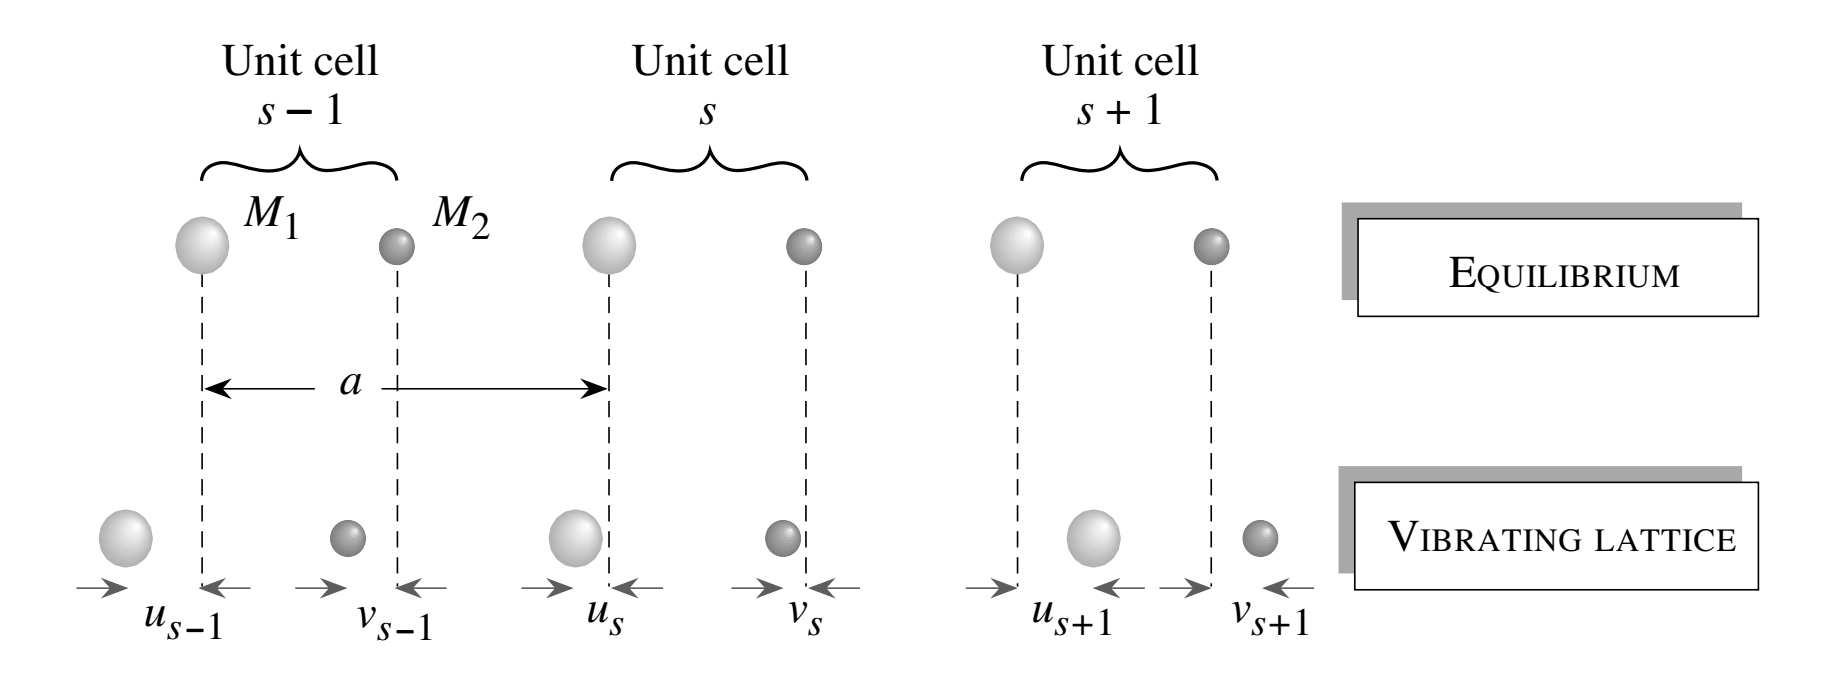
\includegraphics[width=\textwidth]{img/Vibrations.png}
		\\[0.5em]
		\refstepcounter{figure}
		\textbf{Figure~\thefigure.}Lattice vibrations in a crystal with two atoms per unit cell, having masses $M_1$ and $M_2$, connected by a force constant $C$ between adjacent atomic planes.
		\label{fig:Potential_Energy}
	\end{minipage}
\end{center}
We look for traveling wave solutions with alternating amplitudes:
\begin{align}
	u_s & = u \, e^{i s k a} e^{-i \omega t} \\
	v_s & = v \, e^{i s k a} e^{-i \omega t}
\end{align}
Here, \( a \) is the distance between identical planes of atoms (i.e., the lattice periodicity). Substituting into the equations of motion gives:
\begin{align}
	-\omega^2 M_1 u & = C v [1 + e^{-ika}] - 2C u \\
	-\omega^2 M_2 v & = C u [1 + e^{ika}] - 2C v
\end{align}
These form a set of coupled eigenvalue equations, which can be represented in matrix form:
\[
	\begin{pmatrix}
		2C - \omega^2 M_1 & -C(1 + e^{-ika})  \\
		-C(1 + e^{ika})   & 2C - \omega^2 M_2
	\end{pmatrix}
	\begin{pmatrix}
		u \\
		v
	\end{pmatrix}
	= 0
\]
The determinant of this system must vanish:
\[
	\left|
	\begin{matrix}
		2C - \omega^2 M_1 & -C(1 + e^{-ika})  \\
		-C(1 + e^{ika})   & 2C - \omega^2 M_2
	\end{matrix}
	\right| = 0
\]
Expanding and simplifying:
\begin{equation}
	M_1 M_2 \omega^4 - 2C (M_1 + M_2) \omega^2 + 2C^2 (1 - \cos ka) = 0
\end{equation}
Solving this quadratic in \( \omega^2 \), we obtain:
\begin{equation}
	\omega^2 = \frac{2C (M_1 + M_2) \pm \sqrt{4C^2 (M_1 + M_2)^2 - 8C^2 (1 - \cos ka) M_1 M_2}}{2 M_1 M_2}
\end{equation}
Let us consider two limiting cases:
- For small \( k \) (long-wavelength limit), we obtain:
\begin{align}
	\omega_{\text{acoustic}} & \approx \sqrt{\frac{C/2}{M_1 + M_2}} \, ka                                       \\
	\omega_{\text{optical}}  & \approx \sqrt{\frac{2C}{\mu}} \quad \text{with } \mu = \frac{M_1 M_2}{M_1 + M_2}
\end{align}
- At the Brillouin zone boundary \( k = \pi/a \), the frequencies are:
\begin{align}
	\omega_1 & = \sqrt{\frac{2C}{M_1}} \\
	\omega_2 & = \sqrt{\frac{2C}{M_2}}
\end{align}
This analysis yields two distinct branches of lattice vibrations:
\begin{itemize}
	\item The \textit{acoustic branch}, where \( \omega \to 0 \) as \( k \to 0 \), representing sound wave propagation.
	\item The \textit{optical branch}, where \( \omega \) remains finite as \( k \to 0 \), corresponding to out-of-phase motion of the two atoms.
\end{itemize}
The acoustic mode has a linear dispersion relation near \( k = 0 \), and the group velocity (sound speed) is given by:
\begin{equation}
	v_s = \left. \frac{d\omega}{dk} \right|_{k \to 0} = a \sqrt{\frac{C}{M}}, \quad \text{with } M = \frac{M_1 + M_2}{2}
\end{equation}
It is important to examine the eigenfunctions (i.e., the displacement amplitudes \( u_s \)) corresponding to the optical and acoustic branches of the dispersion relation.
For \( k = 0 \), in the case of the \textit{optical branch}, the angular frequency is given by:
\begin{equation}
	\omega^2 = 2C \left( \frac{1}{M_1} + \frac{1}{M_2} \right)
\end{equation}
\begin{center}
	\begin{minipage}{0.8\textwidth}
		\centering
		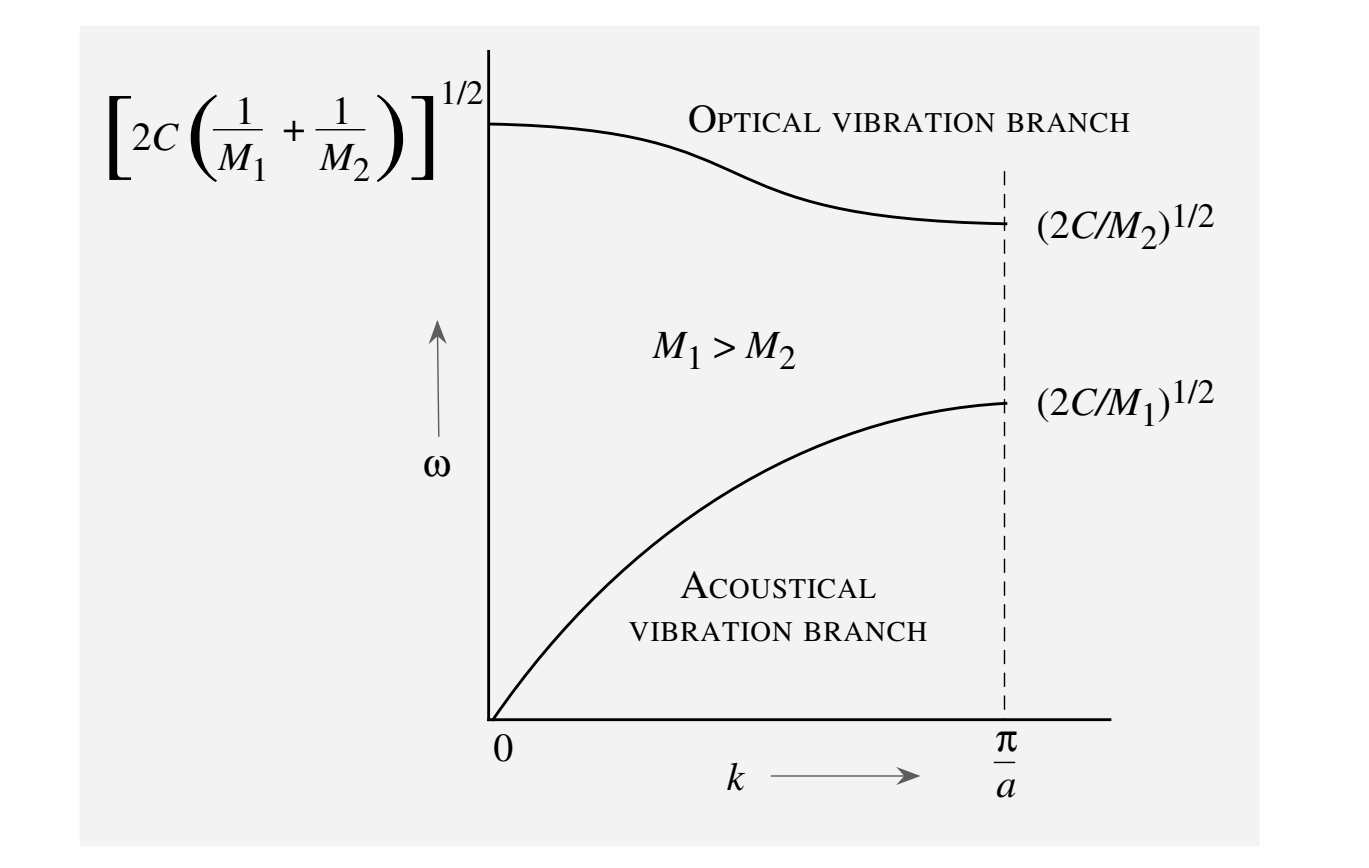
\includegraphics[width=\textwidth]{img/OpticalVSAcoustic_differences.png}
		\\[0.5em]
		\refstepcounter{figure}
		\textbf{Figure~\thefigure.}
		\label{fig:OpticalVSAcoustic_differences}
	\end{minipage}
\end{center}
Substituting this value into the equation of motion, we obtain the relation between the amplitudes of the atomic displacements:
\begin{equation}
	u = -\frac{ M_2}{M_1} v
\end{equation}
In this case, the two atoms vibrate against each other, such that their center of mass remains stationary. This describes an out-of-phase motion, which is characteristic of optical phonons.
In contrast, for the \textit{acoustic branch}, in the long-wavelength limit (\( k \to 0 \)), the solution leads to:
\begin{equation}
	u = v
\end{equation}
This corresponds to both atoms moving in phase, i.e., the entire lattice unit oscillates as a whole, which is characteristic of sound wave propagation.
Furthermore, for each wavevector \( k \), there exist three possible vibrational modes:
\begin{itemize}
	\item One \textbf{longitudinal mode}, where atomic displacements are parallel to the direction of wave propagation.
	\item Two \textbf{transverse modes}, where atomic displacements are perpendicular to the direction of wave propagation.
\end{itemize}
In general, these modes have different frequencies because the restoring forces differ for longitudinal and transverse motions.\\
In ionic crystals such as GaAs, the \textit{optical vibrations} induce oscillating dipole moments due to the displacement of positive and negative ions relative to each other. These polarization fields interact with the vibrations, especially in the longitudinal mode. This interaction introduces an additional long-range restoring force for the longitudinal optical (LO) phonons, increasing their frequency relative to the transverse optical (TO) phonons.\\
As a result, in such materials, the LO phonon frequency is greater than the TO phonon frequency at the zone center (\( k = 0 \)). This splitting is a fundamental feature of polar optical phonons in ionic semiconductors.
\begin{center}
	\begin{minipage}{0.9\textwidth}
		\centering
		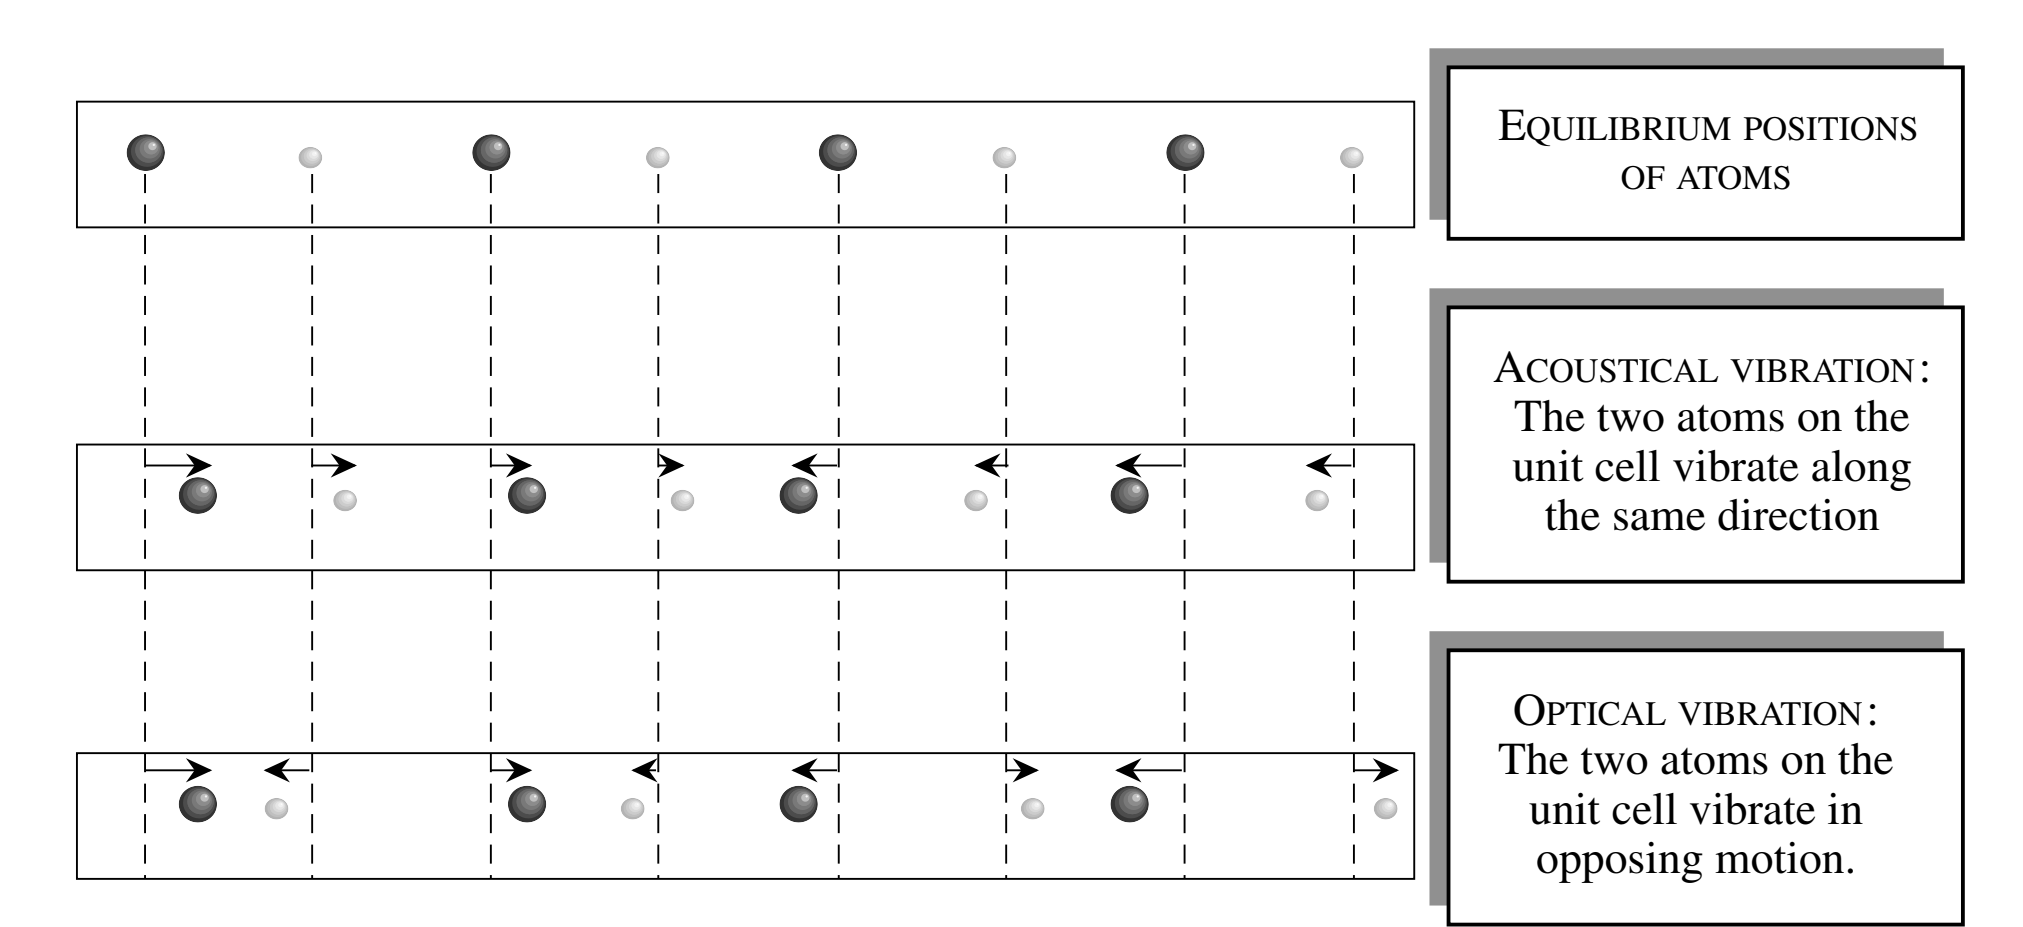
\includegraphics[width=\textwidth]{img/acoustic&opticalmode.png}
		\\[0.5em]
		\refstepcounter{figure}
		\textbf{Figure~\thefigure.}Difference between as acoustical mode an optical mode.
		\label{fig:OpticalVSAcoustic_differences}
	\end{minipage}
\end{center}

\subsection{Phonon: Quantization of Lattice Vibrations}
In the previous discussions, we evaluated the dispersion relation \( \omega \) vs. \( k \) for a set of coupled harmonic oscillator equations. If we now consider a single harmonic oscillator problem in quantum mechanics with the Hamiltonian:
\begin{equation}
	H = \frac{P^2}{2m} + \frac{1}{2} C x^2
\end{equation}
\noindent
the energy of the vibrating particle is quantized and given by:
\begin{equation}
	\epsilon_n = \left(n + \frac{1}{2}\right)\hbar\omega, \quad n = 0, 1, 2, \dots
\end{equation}
\noindent
where \( \omega = \sqrt{C/m} \) is the classical frequency of oscillation.
In classical physics, the oscillator energy can vary continuously with the amplitude of vibration. However, in quantum mechanics, the oscillator has a minimum energy of \( \hbar \omega / 2 \) and its energy increases in discrete steps of \( \hbar \omega \).
In the framework of second quantization, the integer \( n \) represents the number of "particles" or quanta of vibrational energy in the system. These quanta are called \textit{phonons}. A phonon is the quantized mode of lattice vibration, analogous to how a photon is the quantum of light.\\
For a single oscillator, the frequency \( \omega \) is fixed. However, in a crystal made up of many coupled atoms (i.e., coupled oscillators), the vibrational frequencies span a range. These are indexed by a wavevector \( k \), leading to a dispersion relation \( \omega(k) \). The quantized energy for a given wavevector \( k \) is:
\begin{equation}
	\epsilon_k = \left(n_\mathbf{k} + \frac{1}{2}\right) \hbar \omega_\mathbf{k}
\end{equation}
\noindent
where \( n_\mathbf{k} \) is the number of phonons in the mode with wavevector \( \mathbf{k} \) and frequency \( \omega_\mathbf{k} \).\\
To determine how many phonons occupy a given mode, we will later define the appropriate statistical distribution for phonons.
The allowed wavevectors \( k \) in a crystal with \( N \) unit cells and periodic boundary conditions are given by:
\begin{equation}
	|\mathbf{k}| = \frac{2\pi n}{Na}, \quad n = 0, \pm 1, \dots, \pm \left(\frac{N}{2} - 1\right)
\end{equation}
\noindent
This quantization implies there are a total of \( 3N \) vibrational modes in the crystal: \( N \) longitudinal and \( 2N \) transverse modes. Each mode can have an integer occupation number \( n_k \) determined by phonon statistics.


\section{Phonon Statistics}
We have briefly introduced the concept that lattice vibrations can be quantized in terms of particles known as $k$-phonons. To determine how many phonons occupy a specific vibrational mode with angular frequency $\omega$ at a given temperature $T$, one must consider the relevant statistical distribution. Phonons, being bosonic in nature, are governed by Bose–Einstein statistics under conditions of thermal equilibrium.\\
The average phonon number in a mode with frequency $\omega$ is expressed as:
\begin{equation}
	\langle n_{\omega} \rangle = \frac{1}{\exp\left( \frac{\hbar \omega}{k_B T} \right) - 1}
\end{equation}
\begin{center}
	\begin{minipage}{0.5\textwidth}
		\centering
		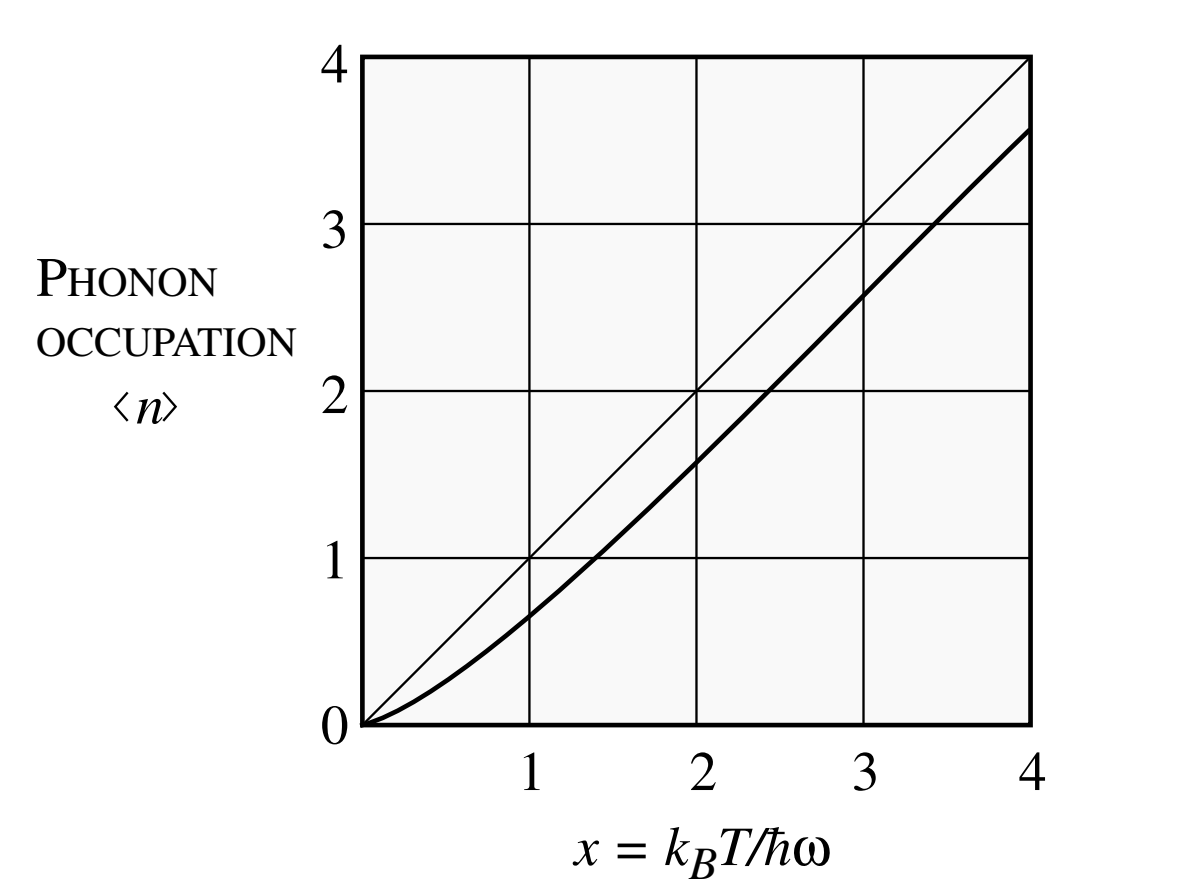
\includegraphics[width=\textwidth]{img/BoseEinstein_distribution.png}
		\\[0.5em]
		\refstepcounter{figure}
		\textbf{Figure~\thefigure.} Bose-Einstein distribution.
		\label{fig:BoseEinstein_distribution}
	\end{minipage}
\end{center}
Unlike electrons, whose occupancy follows the Fermi–Dirac distribution and is restricted to at most one particle per state, bosons such as phonons are permitted to share quantum states. Consequently, the occupation number for phonons can exceed unity. As temperature increases, lattice vibrations become more intense, leading to a higher average phonon population, $\langle n_{\omega} \rangle$.\\
It is worth highlighting that at lower temperatures, the occupation of optical phonons remains minimal due to their relatively high energy at any wavevector $k$. In contrast, acoustic phonons, which can have very small $\hbar \omega$ values at low $k$, maintain significant occupancy even at low temperatures. Therefore, optical phonons contribute less significantly at low temperatures.\\
In the limiting case where $\hbar \omega \ll k_B T$, the phonon occupation number simplifies to:
\begin{equation}
	\langle n \rangle \approx \frac{k_B T}{\hbar \omega}
\end{equation}
The total energy associated with the lattice vibrations, neglecting the zero-point energy, is given by summing over all wavevectors $k$ and polarizations $\rho$:
\begin{equation}
	U = \sum_{\mathbf{k}, \rho} \langle n_{\mathbf{k}, \rho} \rangle \hbar \omega_{\mathbf{k}, \rho}
\end{equation}
Here, $\mathbf{k}$ represents the phonon wavevector and $\rho$ denotes the polarization index of each vibrational mode.

\subsection{Conservation Laws in Scattering of Particles involving Phonons}
A phonon characterized by a wave vector $\mathbf{k}$ can interact with other particles such as electrons or photons, imparting momentum as though it carries a value $\hbar \mathbf{k}$. It is important to recall that for electrons, the quantity $\hbar \mathbf{k}$ (related to the wave vector) represents the relevant momentum, rather than the actual mechanical momentum of the particle. Although phonons are treated as if they possess momentum, they do not carry any real physical momentum. This is because lattice vibrations involve atoms oscillating about their equilibrium positions in opposite directions, meaning the overall motion of the crystal remains unchanged. Thus, the net physical momentum associated with lattice vibrations is zero.\\
This can also be demonstrated mathematically. The total momentum of the crystal can be expressed as:
\begin{equation}
	\mathbf{p} = M \frac{d}{dt} \sum_s \mathbf{u}_s
\end{equation}
where $M$ is the total mass and $\mathbf{u}_s$ denotes the displacement of atom $s$. Given the form of the vibrational solution, this summation evaluates to zero, which aligns with the physical expectation that the center of mass of the crystal does not move.\\
When examining electron-phonon interactions, it is found that first-order phonon scattering processes must obey conservation laws. Specifically, the conservation of crystal momentum and energy leads to the following relations:
\begin{equation}
	\mathbf{k}_i = \mathbf{k}_f \pm \mathbf{q}
\end{equation}
\begin{equation}
	\mathbf{E}_i = \mathbf{E}_f \pm \hbar \omega_{\mathbf{q}}
\end{equation}
Here, $\mathbf{k}_i$ and $\mathbf{k}_f$ represent the initial and final wave vectors of the electron, $\mathbf{q}$ is the phonon wave vector, and $\mathbf{E}_i$, $\mathbf{E}_f$, and $\hbar \omega_{\mathbf{q}}$ correspond to the respective energies involved. For more intricate scattering events involving multiple phonons, these conservation laws are extended accordingly to account for the additional complexity.

\section{Polar Optical Phonons}
In previous discussions concerning optical phonons, we have not accounted for the fact that, in certain semiconductors, the constituent atoms possess net charges—specifically, positive and negative ions such as cations and anions. This ionic characteristic is not present in group IV elemental semiconductors like Si, Ge, or C. However, in compound semiconductors, the ionic nature gives rise to an additional restoring force due to long-range polarization fields that accompany lattice vibrations.
\begin{center}
	\begin{minipage}{0.8\textwidth}
		\centering
		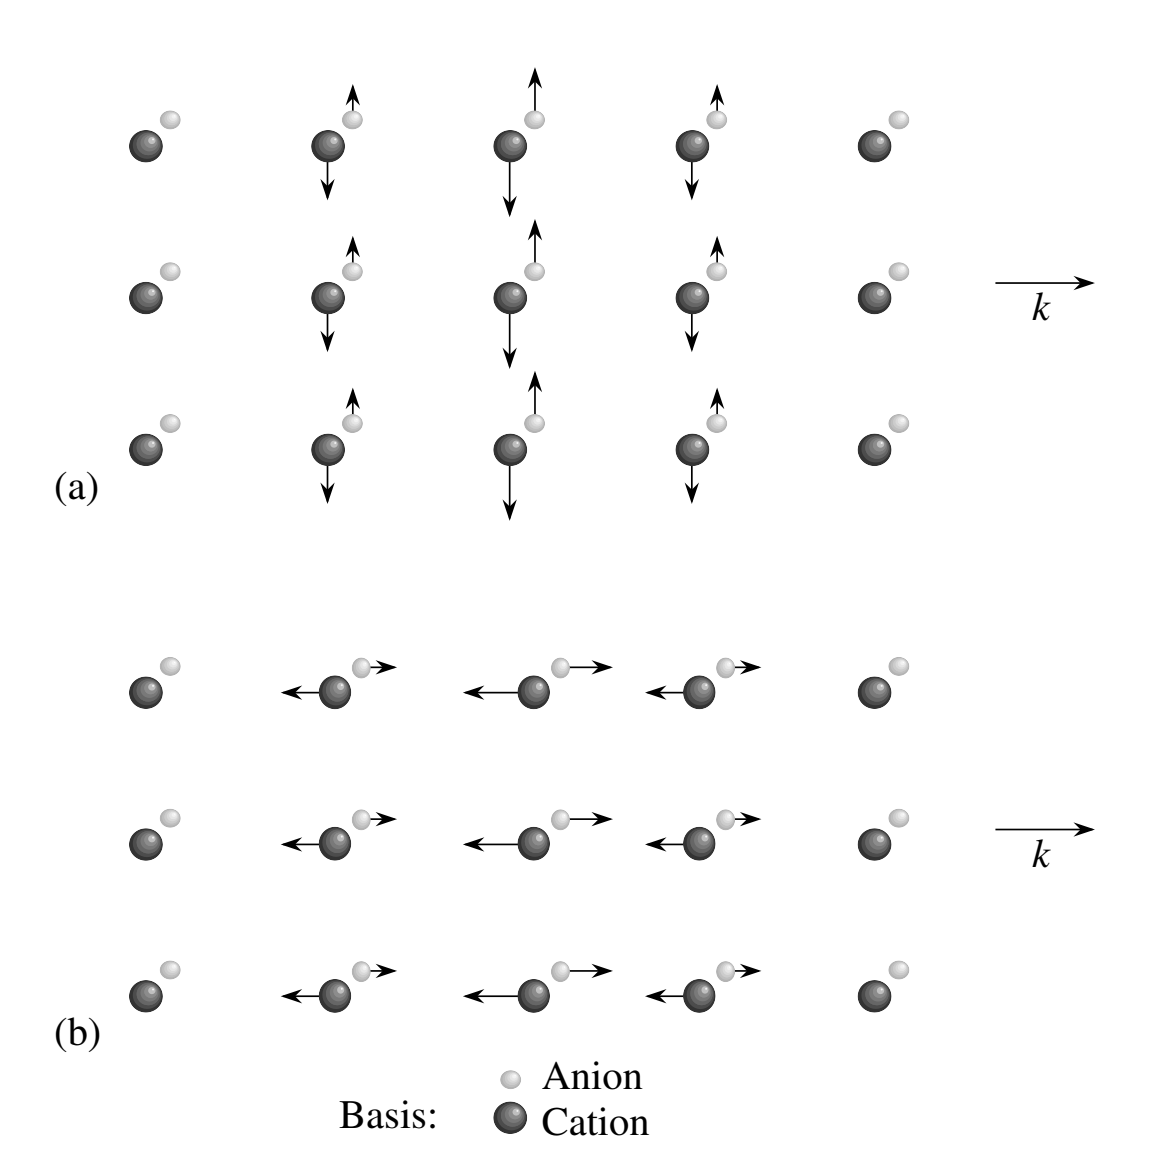
\includegraphics[width=\textwidth]{img/OpticalModes.png}
		\\[0.5em]
		\refstepcounter{figure}
		\textbf{Figure~\thefigure.} Optical vibrations in an ionic crystal.(a) Transverse optical modes do not induce macroscopic polarization. (b) Longitudinal optical modes generate long-range electric fields due to polarization effects.

		\label{fig:OpticalModes}
	\end{minipage}
\end{center}
To examine this phenomenon, we consider two conceptual approaches. The first, although highly simplified, effectively illustrates the essential physical concepts. We work in terms of the relative displacement vector
\begin{equation}
	\mathbf{u}_r = \mathbf{u} - \mathbf{v}
\end{equation}
which denotes the relative motion between the sublattices of positively and negatively charged ions. For transverse vibrational modes, which do not generate macroscopic polarization, the equation of motion takes the form
\begin{equation}
	M \ddot{\mathbf{u}}_r + M \omega_t^2 \mathbf{u}_r = 0
\end{equation}
where $M$ is the reduced mass of the two atoms, and $\omega_t$ is the transverse optical phonon frequency.\\
In contrast, longitudinal vibrational modes induce an electric field as a result of polarization. The equation of motion in this case incorporates both the mechanical restoring force and the force due to the induced electric field, yielding
\begin{equation}
	- \omega_l^2 M \mathbf{u}_r = - \omega_t^2 M \mathbf{u}_r + \mathbf{F}_i e^*
\end{equation}
Here, $\mathbf{F}$ represents the internal electric field generated by polarization, and $e^*$ is an effective charge per ion. Assuming $n$ unit cells per unit volume, the polarization is given by
\begin{equation}
	\mathbf{P} = n e^* \mathbf{u}_r
\end{equation}
The associated electric field in a vacuum, using $\varepsilon_0$ as the permittivity of free space, is
\begin{equation}
	\mathbf{F} = -\frac{\mathbf{P}}{\varepsilon_0} = -\frac{n e^* \mathbf{u}_r}{\varepsilon_0}
\end{equation}
Substituting this into the equation of motion leads to a corrected expression for the longitudinal optical phonon frequency:
\begin{equation}
	\omega_l^2 = \omega_t^2 + \frac{n {e^*}^2}{\varepsilon_0 M}
\end{equation}
If the material possesses a static relative dielectric constant $\varepsilon_r$ such that $\varepsilon = \varepsilon_r \varepsilon_0$, the equation becomes
\begin{equation}
	\omega_l^2 = \omega_t^2 + \frac{n \epsilon_{rel} {e^*}^2}{M \varepsilon_0}
\end{equation}
The effective charge $e^*$ will be addressed further in the context of polar optical phonon scattering. It should be noted that the longitudinal optical phonon frequency exceeds that of the transverse phonons near the Brillouin zone center ($k \approx 0$). In group IV elemental semiconductors, no such frequency splitting exists at $k = 0$ due to the absence of ionicity. However, in III–V compound semiconductors, the difference becomes significant because of their polar nature.\\
An important observation is that optical phonons exhibit minimal dispersion near $k = 0$; their energy bands are nearly flat, unlike those of acoustic phonons. Accordingly, in future discussions on electron-phonon scattering, we will assume that optical phonons are dispersionless.

\section{Phonons in Heterostructures}
It is evident that the behavior of phonons bears a strong resemblance to that of electrons, as both phenomena involve solving differential equations within a periodic potential. In the context of heterostructures, the concept of electronic band structure has already been explored, particularly in relation to systems such as quantum wells and superlattices. These same structural configurations exert a notable influence on phonon dispersion, much like their effect on electronic spectra.\\
The distinction between the electronic and phononic cases, however, lies primarily in the characteristic length scales involved. For electrons, the band offsets in semiconductors give rise to heterostructure effects when the quantum well dimensions approach the electron de Broglie wavelength, typically on the order of 100~\AA. In contrast, for phonons, the relevant length scales are considerably shorter—on the order of a few monolayers.\\
Consequently, there exist phonon modes that are uniquely associated with interfaces and with superlattices of narrow periodicity. These interface-related phonon modes can play a significant role in determining the thermal and vibrational properties of the heterostructure.
\subsection{Confined Optical Phonons}
In superlattices with narrow periodicity, phonon modes can become confined within individual layers, in much the same way that electron wavefunctions are confined within a quantum well. A notable example of this occurs in systems composed of alternating layers of GaAs and AlAs. The optical phonon dispersion relations of these two materials do not intersect, implying that optical modes originating in one material are unable to propagate into the adjacent layer. As a result, these phonon modes are spatially confined to their respective layers.

This confinement leads to a situation analogous to a particle in an infinite square potential well. The permitted wave vectors for such confined modes are quantized according to the relation
\begin{equation}
	|k_n| = \frac{n}{2d}, \quad \text{for } n = 1, 2, 3, \dots
\end{equation}
where $d$ denotes the thickness of the individual GaAs or AlAs layer. Remarkably, the energies of these confined phonon modes have been observed to closely follow the dispersion curves of the corresponding bulk materials. That is, the function $E(k)$ remains nearly unchanged whether evaluated at the continuous $k$ values characteristic of bulk GaAs or at the discrete $k$ values dictated by quantization within the confined layer.
\subsection{Interface Phonons}
In semiconductor heterostructures, there also exist vibrational modes within the optical phonon frequency range that are characterized by having their maximum amplitude localized at the interfaces between two distinct materials. These so-called interface modes are of particular interest because they are accompanied by macroscopic electric fields.
Such modes can be effectively understood using a simplified electrostatic model. The discontinuity in material properties across the interface—such as dielectric constants and ionic character—gives rise to polarization effects, which in turn generate electric fields associated with the vibrational modes.\\

\section{Phonon Scattering: General Formalism}
In our treatment of electronic bandstructure, we have assumed a static, time-independent periodic potential as the background. This assumption enables the derivation of electronic bands. In contrast, lattice vibrations introduce a time-dependent aspect to the crystal potential, leading to the quantized vibrational excitations known as phonons and their associated dispersion relations.\\
The possibility of separating, at first order, the electronic behavior from lattice dynamics relies on the validity of the adiabatic approximation. This approximation is applicable to systems where the time dependence of the Hamiltonian evolves slowly enough that, at each instant, the system can be regarded as effectively time-independent. While phonon frequencies fall in the terahertz range—on the order of $10^{12}$ Hz—this still qualifies as “slow” compared to electronic time scales due to the large difference in mass between electrons and nuclei. As such, the adiabatic approximation proves to be highly effective, allowing us to proceed in two distinct stages:
\begin{enumerate}
	\item Determine the electronic states in a perfect lattice, yielding the electronic bandstructure.
	\item Analyze the interactions between electrons and lattice vibrations, or phonon scattering.
\end{enumerate}
In previous sections, it has been shown that in semiconductors with two atoms per basis, both acoustic and optical phonon modes arise. Near the Brillouin zone center ($k = 0$), acoustic phonons exhibit a linear relationship between $\omega$ and $k$, while optical phonons are nearly dispersionless. Each of these types of phonons exists in both longitudinal and transverse polarization modes. The motion of atoms within the lattice produces strain, which, according to deformation potential theory, leads to perturbations in the electronic energy levels. This relationship has already been explored in the context of strain-induced modifications to bandstructure.\\
Generally, the interaction between electrons and phonons depends on the atomic displacement $\mathbf{u}$. The resulting perturbation potential $U$ takes different forms depending on the type of phonon:
\begin{align*}
	\text{Acoustic phonons:} \quad            & U \sim D \frac{\partial u}{\partial x} \\
	\text{Optical phonons (non-polar):} \quad & U \sim D_0 u                           \\
	\text{Polar optical phonons:} \quad       & U \sim e^* u
\end{align*}
Here, $e^*$ is an effective charge per ion.\\
\begin{center}
	\begin{minipage}{0.5\textwidth}
		\centering
		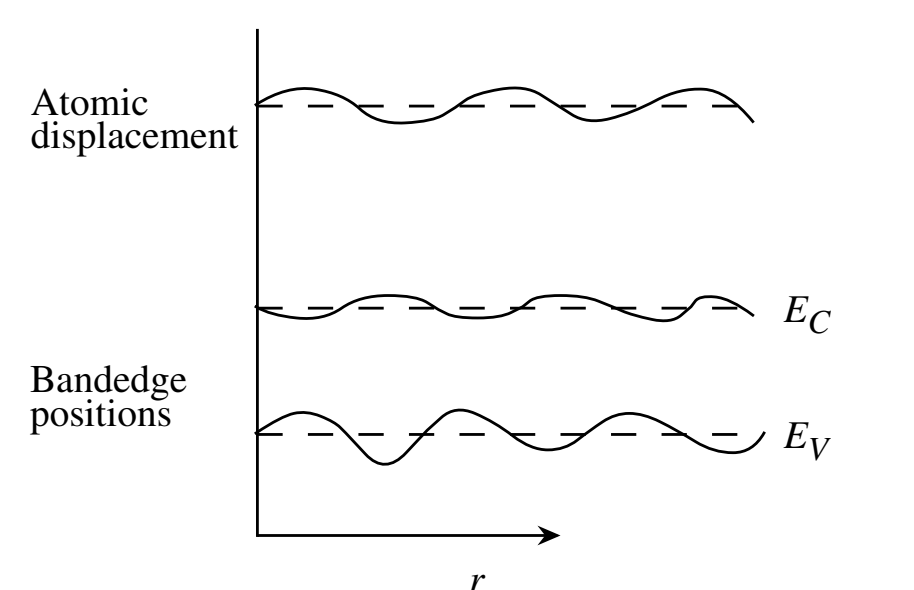
\includegraphics[width=\textwidth]{img/AtomicDisplacements.png}
		\\[0.5em]
		\refstepcounter{figure}
		\textbf{Figure~\thefigure.} Effect of atomic displacements on bandaedge energy levels in real space.
		\label{fig:AtomicDisplacements}
	\end{minipage}
\end{center}
To describe the scattering of electrons by lattice vibrations, we invoke the framework of second quantization. In this formalism, classical vibrational modes are quantized and described by phonons—quanta of vibrational energy. A harmonic oscillator with frequency $\omega$ has quantized energy levels given by
\begin{equation}
	E = \left( n + \frac{1}{2} \right) \hbar \omega
\end{equation}
where $n$ is the number of phonon quanta. The phonon number operator is defined as $n = a^\dagger a$, with $a^\dagger$ and $a$ being the phonon creation and annihilation operators, respectively. These operators satisfy the following relations:
\begin{equation}
	a |n\rangle = \sqrt{n} |n-1\rangle, \quad a^\dagger |n\rangle = \sqrt{n+1} |n+1\rangle
\end{equation}
The displacement and momentum operators in terms of $a$ and $a^\dagger$ are:
\begin{align*}
	u = \sqrt{\frac{\hbar}{2 M \omega}} (a + a^\dagger), \quad
	p = i \sqrt{\frac{M \hbar \omega}{2}} (a^\dagger - a)
\end{align*}
These expressions allow us to understand electron-phonon interactions in terms of phonon creation (emission) and annihilation (absorption) processes. In the quantum description, the emission of a phonon corresponds to the application of the creation operator, while absorption corresponds to the action of the annihilation operator.\\
Since the lattice vibrational system consists of many coupled oscillators, the physical displacement $\mathbf{u}$ representing atomic motion must be expressed in terms of normal coordinates—modes in which the vibrations are uncoupled. This transformation enables each mode to be treated as an independent harmonic oscillator. The displacement field can thus be written as
\begin{equation}
	\mathbf{u} = \frac{1}{\sqrt{N}} \sum_{\mathbf{q}} \left[\theta_{\mathbf{qb}} \mathbf{b}_\mathbf{q} e^{i \mathbf{q} \cdot \mathbf{R}}  + c.c. \right]
\end{equation}
where $q$ is the phonon wavevector, $b$ indexes the phonon branches, $\theta_b$ is the normal mode amplitude, and $N$ is the number of unit cells. This formalism provides the foundation for analyzing phonon-mediated scattering processes in semiconductors.
\begin{center}
	\begin{minipage}{0.9\textwidth}
		\centering
		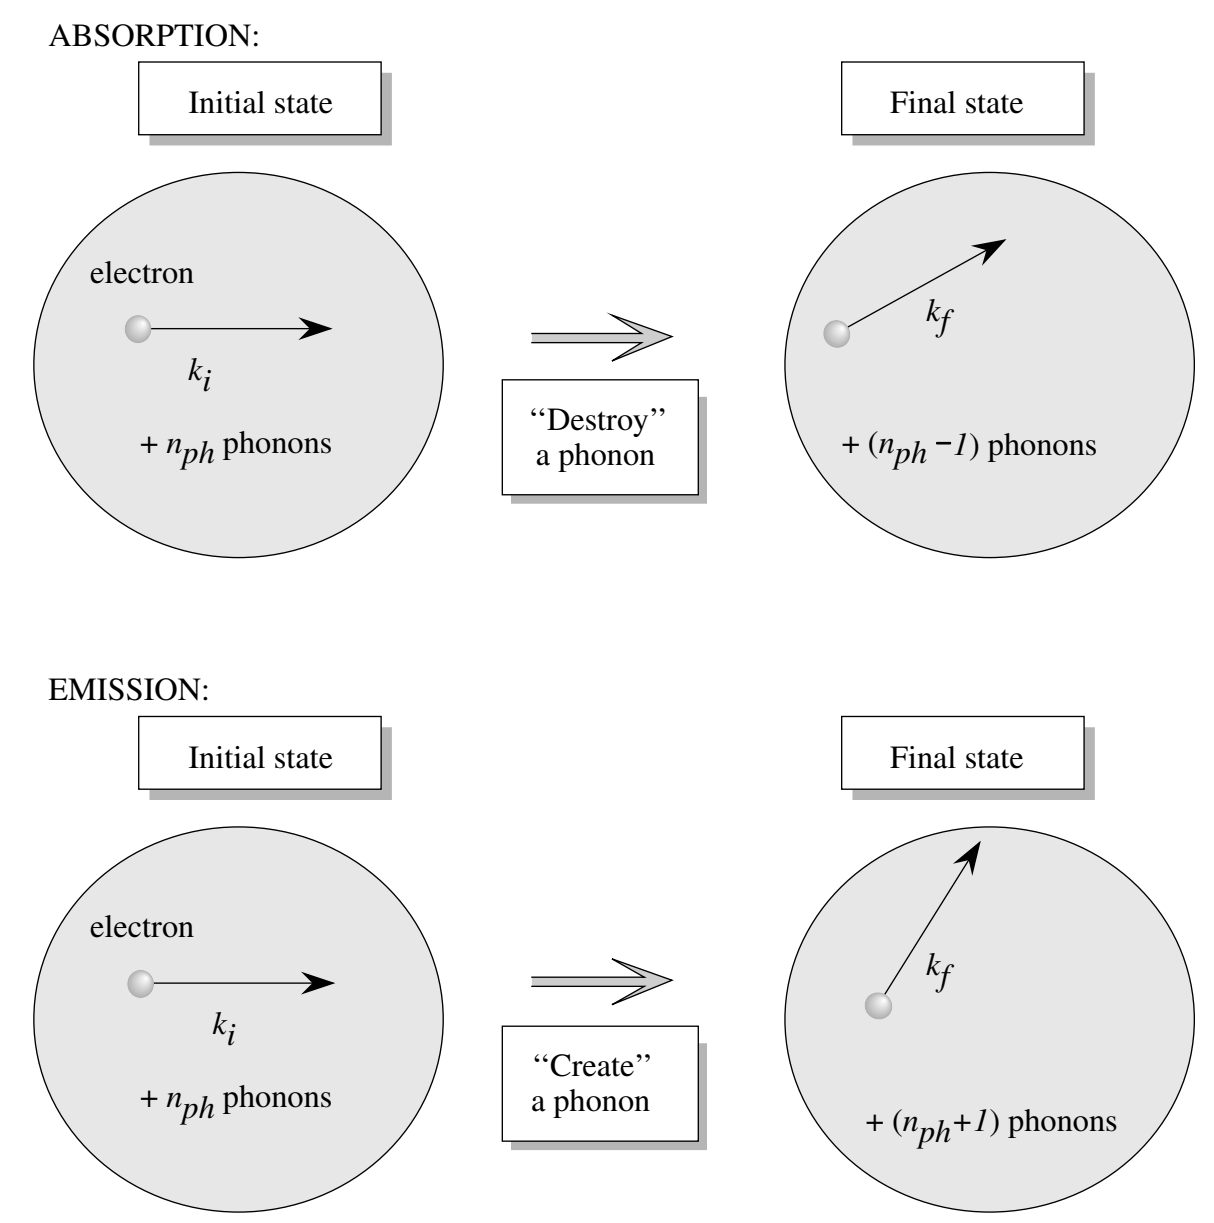
\includegraphics[width=\textwidth]{img/absandemission_phonon.png}
		\\[0.5em]
		\refstepcounter{figure}
		\textbf{Figure~\thefigure.} (a) Schematic of a phonon absorption process, where a phonon is annihilated and the electron's energy and momentum change accordingly. (b) Schematic of a phonon emission event, where a phonon is generated as the electron loses energy.
		\label{fig:absandemission_phonon}
	\end{minipage}
\end{center}

The two fundamental phonon-related processes involved in electron–phonon interactions correspond to the annihilation and creation of phonons. These are commonly referred to as \textbf{phonon absorption} and \textbf{phonon emission}, respectively.\\
In the quantum mechanical treatment of lattice vibrations, the interaction Hamiltonian includes two terms within the brackets. The first term represents the removal of a phonon from the initial state during the scattering process—this corresponds to \textbf{phonon absorption}. The second term accounts for the addition of a phonon to the final state—this is the \textbf{phonon emission} process.\\
A key distinction between the two processes arises from the phonon occupation number. Phonon absorption requires that a phonon be present initially; thus, if the initial phonon population is zero, the probability of absorption vanishes. In contrast, the emission process involves a factor of $(n + 1)$, meaning that emission can occur even in the absence of initial phonons, due to spontaneous emission.\\
At thermal equilibrium, the average phonon occupation number follows Bose–Einstein statistics.